\section{Astrodynamics \& control tool development}
\label{ch:astrocontrol}
In this chapter the development of a tool for astrodynamics and control is described. The tool calculates the trajectory of the spacecraft for varying initial conditions and aerodynamic properties. With the information extracted from this tool requirements**maybe requirements is not the right word** for the control systems can be determined. Based on these requirements the different control systems available for the different concepts (which are presented in chapter \ref{ch:options}) can be weighed off in a trade-off in chapter \ref{ch:tradeoff}.

In this chapter first the purpose of the tool will be explained in section \ref{sec:astropurpose}. In sections \ref{sec:astrogov} and \ref{sec:astrowp} working principles of the tool are explained and the equations the tool is based on are presented. To ensure the tool calculates what it is supposed to calculate and to ensure this happens accurately enough in section \ref{sec:astrovv} the verification and validation of the tool is done. In section \ref{sec:astroref} performance of current day control systems are investigated. This performance is compared to the calculated needed performance to come to a conclusion in section \ref{sec:astrores}. Section \ref{sec:astrores} also presents some other results of the tool which are used as input for tools calculating i.e. structural mass.

\subsection{Purpose of tool development}
\label{sec:astropurpose}
The purpose of developing a tool to calculate the trajectory of the spacecraft during entry is firstly to know the trajectory of the spacecraft given its characteristics. Secondly, calculating trajectories for varying input, for the different concepts and different control systems, this tool can also give an insight in which concepts have the characteristics needed for a successful entry.

The tool has been developed in-house as no existing tool that both suits our purpose and is publicly available has been found.

More specifically the tool is used here to determine the required Aerodynamic characteristics to create an acceptable window of entry. Or in other words: What accuracy of the initial conditions is needed to, with a certain shape and control, get the required accuracy at the final position. Taking into account the different shapes the goal of this tool is to investigate the need for \& effect of control on the trajectory of the spacecraft.

\subsection{Governing equations}
\label{sec:astrogov}
In this section the equations on which the tool is based are shown and the reason for using them is explained. The trajectory is split up into three parts: hyperbolic kepler entry, trajectory in atmosphere and eliptic kepler orbit. These are parts presented respectively in sections \ref{sec:hypkep}, \ref{sec:trajatmos} and \ref{sec:eliptickep} respectively. However first all assumptions made are stated in section \ref{sec:astroassumption}.

\subsubsection{Assumptions}
 \label{sec:astroassumption}
 In this section all assumptions used to create the tool are stated and justified. Some of the assumprions have a big impact and should be taken into account in next versions of the program, this are the primary assumptions. There are however also some assumptions that have a negligable effect on the results, this are the secondary assumptions. The list of assumption beneath is subdivided in these catagories.
 
 \paragraph{primary assumptions}
 \begin{itemize}
 \item All atmospheric properties only vary with the height above MOLA ***source*** and not with longitude, latitude or time. This assumption induces a significant error in the output of the tool. However implementing a variable atmosphere adds a lot of complexity aswell. For example the longitude and latitude of initial entry will also become design variables
 \item 
 \end{itemize}
 
 
 \paragraph{secondary assumptions}
 \begin{itemize}
 \item The spacecraft is assumed to only feel a gravitational pull from mars. It is thus assumed that there is no gravitational pull from the sun, any other planet or the martian moons.
 \item The atmosphere stops at a height of 400 $\left[km\right]$. At this point the atmosphere is negligibly thin, adding any more atmosphere would not contribute significantly to the results.
 \end{itemize}
 
\subsubsection{Hyperbolic Kepler entry}
 \label{sec:hypkep}
Before initial entry into the atmosphere the spacecraft follows a hyperbolic Kepler trajectory untill it reaches the atmosphere. From the initial conditions a new position, velocity and acceleration need to be found. 

First the Keplerian orbit parameters need to be determined. For this calculations the known initial conditions are used. The eccentricity $\left(\gls{sym:e}\right)$ can be calculated by Kepler's second law, which is expressed in a formula in equation \ref{eq:kep2nd}.

\begin{equation}
\frac{dA}{dt} = \frac{1}{2}\sqrt{a\gls{con:mu}(1-e^2)}
\label{eq:kep2nd}
\end{equation}
Where $\frac{dA}{dt} = \frac{1}{2}r(t)r(t+dt)*\sin{d\gls{sym:phi}}$.

The semi-major axis $\left(\gls{sym:a}\right)$ can be extracted from the Vis-Viva equation, which is shown in equation \ref{eq:visviva}.

\begin{equation}
\gls{sym:V}^2 = \gls{con:mu}\left(\frac{2}{\gls{sym:R}}-\frac{1}{\gls{sym:a}}\right)
\label{eq:visviva}
\end{equation}

From the initial position an angle \gls{sym:phi} wrt the hyperbolic reference frame can be calculated with equation \ref{eq:polarkep}. In the inertial reference frame the angle of the spacecraft can also be calculated. Using both angles an offset of the hyperbolic frame from the initial frame$\left (\gls{sym:phip}\right)$ can be calculated.

\begin{equation}
\gls{sym:R} = \frac{\gls{sym:a}(1-\gls{sym:e}^2)}{1+\gls{sym:e}\cos{\gls{sym:phi}}}
\label{eq:polarkep}
\end{equation}

With the Keplerian orbital parameters and \gls{sym:R} on the edge of the atmosphere known. Using equation \ref{eq:visviva} the new magnitude of the \gls{sym:V} can be calculated. The direction of \gls{sym:Vv} has been determined based on the tangent to the hyperbola (calculated in the hyperbolic frame) rotated over an angle \gls{sym:phip}.

The direction of \gls{sym:Rv} is based on \gls{sym:phi}, which is calculated with equation \label{eq:polarkep} where \gls{sym:R} is known.

The acceleration $\left(\gls{sym:acc}\right)$ is only the gravitational pull $\left(\gls{sym:g}\right)$, which can be calculated with equation \ref{eq:grav}.

\begin{equation} \label{eq:grav}
\gls{sym:g} = -\frac{\gls{con:G}\gls{con:Mmars}}
					{\gls{sym:R}^3}\gls{sym:Rv}
\end{equation}

\subsubsection{Trajectory in atmosphere}
 \label{sec:trajatmos}
***Forces give accelerations: like in baseline + Jerk***\\

\subsubsection{Eliptical Kepler orbit}
 \label{sec:eliptickep}
For an eliptical orbit \gls{sym:a}, \gls{sym:e} and \gls{sym:phip} can be calculated in the same way as was done in section \ref{sec:hypkep}. The point of reentry into the atmosphere is the old location exactly mirrored in the line between the pericenter and the apocenter. Also the velocity $\left(\gls{sym:Vv}\right)$ and the acceleration $\left(\gls{sym:acc}\right)$  should be mirrored in that line. The velocity should than be rotated over 180 $\left[^\circ\right]$ to point in the correct direction. The magnitude of the location $\left(\gls{sym:R}\right)$, velocity $\left(\gls{sym:V}\right)$ and acceleration $\left(\gls{sym:acc}\right)$ are still the same due to the symmetry of kepler orbits.

For the eliptical orbit also the duration has to be calculated. As this time is part of the 10 days in which the spacecraft is required to decelerate. As keplers second law states: $\frac{dA}{dt}=\mbox{constant}$, the duration can be written as an area fraction of the period. This is done in equation \ref{eq:areatime}. Here $\gls{sym:P} = 2\pi\sqrt{\frac{\gls{sym:a}^3}{\gls{con:mu}}}$ and $\gls{sym:A}_{tot} = 2\pi \gls{sym:a} \sqrt{1-\gls{sym:e}^2}$.

\begin{equation}
t = \frac{\gls{sym:A}}{\gls{sym:A}_{tot}}\gls{sym:P}
\label{eq:areatime}
\end{equation}

\subsection{Working principles of the tool}
\label{sec:astrowp}
The tool is able to calculate the trajectory of the spacecraft and a range of important parameters at each moment in time. These parameters are among others: Acceleration $\left(\gls{sym:acc}\right)$, dynamic pressure $\left(\gls{sym:q}\right)$, speed $\left(\gls{sym:Vv}\right)$ and Mach number $\left(\gls{sym:M}\right)$. In order to calculate this the tool takes geometric and aerodynamic properties of the spacecraft and some initial conditions as input.

***Flowchart + very short explanation***\\

\subsection{Verification \& validation}
\label{sec:astrovv}

In order to be sure the results the tool produces are correct and can safely be used in further efforts to design the \gls{cia} verification and validation is needed. This section presents the methods used to verify and validate the results produced by the tool. First a sensitivity analysis is presented in section \ref{sec:astrosens} which focusses on the sensitivity of the program to the initial conditions. In section \ref{sec:astrodisc} the discretisation error is analysed in order to ensure the results are accurate enough for it to be usefull. The numerical solution is compared to the simple case of a kepler orbit in section \ref{sec:astroverf}. Lastly in section \ref{sec:astroval} the results produced by the tool are compared to data from missions that have flown in the past.

\subsubsection{Sensitivity analysis}
\label{sec:astrosens}

In order to assure 

***sensitivity analysis: very sensitive to initial location, thus for now assumed initial location closer***\\

\subsubsection{Discretisation error}

%Initial Position
%rx = -4143775;
%ry = 10*R_m;
%R = [rx,ry,0];

%Initial Velocity
%v = 7.1679e+03; %[m/s]
%V = [0,-v,0];

\begin{figure}[h]
	\centering
	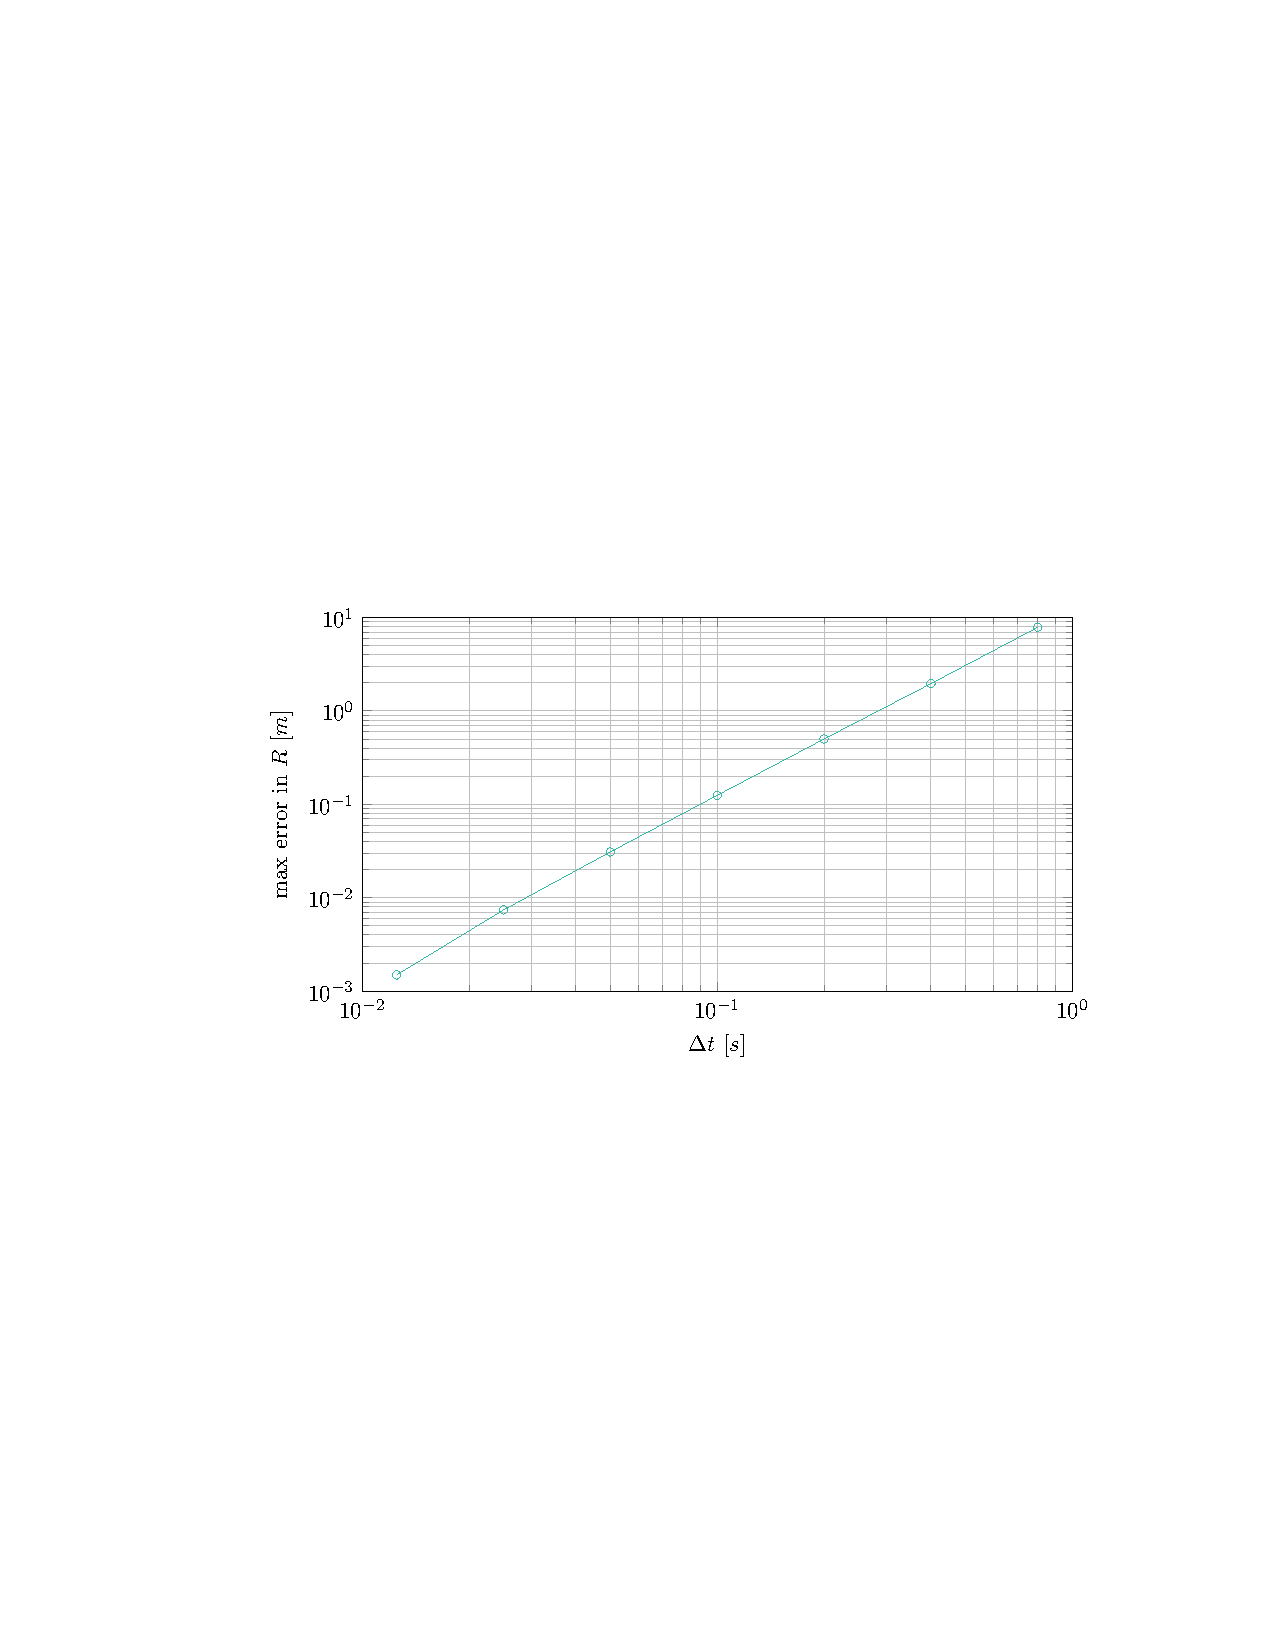
\includegraphics[trim={4.25cm 10cm 3.2cm 10cm},clip,width=0.8\textwidth]{Figure/orbital_model/dicretization.pdf}
	\caption{The atmospheric properties at $50$ $\left[km\right]$} 
	\label{fig:atmos_disc}
\end{figure}

\label{sec:astrodisc}
***discretisation error: error for different dt***\\

\subsubsection{Verification through comparison with kepler}
\label{sec:astroverf}
***Compare numerical results with Kepler, should be the same for rho=0***\\

\subsubsection{Validation through comparison with reference cases}
\label{sec:astroval}
***Validation through checking if output values are approximately the same as reference cases (peak dynamic pressure)***\\

%\subsection{Performance of control systems}
% \label{sec:astroref}
%Several options for the control system are considered. Using first-order calculations the effectiveness of each control system design option will be assessed. In this context 'effectiveness' is defined as a combination of system mass, moment that can be caused by the system and whether a control output can be sustained for long periods of time. These three criteria will be considered for all three control system design options. The design options to be considered are:
%\begin{itemize}
%	\item Shifting the \acrfull{cg}
%	\item A \acrfull{rcs}
%	\item Control surfaces (body flaps)
%\end{itemize}
%Each of these options will be quickly assessed in the subsequent sections. This will be done by taking angle of attack \gls{sym:alpha}$=30\deg$. This corresponds to $\gls{sym:CM}\gls{sym:A}=-100$, $\gls{sym:CL}\gls{sym:A}=-58.8$ and $\gls{sym:CD}\gls{sym:A}=126$. These values have been obtained by using the aerodynamical tool described in chapter \ref{ch:aero_analysis} for an Apollo-shaped object. Using equation \ref{eq:moment_from_cm} the control moment required can be obtained.
%\begin{equation}
%M=\frac{1}{2}\gls{sym:rho}\gls{sym:V}^{2}\gls{sym:CM}\gls{sym:A}
%\label{eq:moment_from_cm}
%\end{equation}
%This moment has to be counteracted during a time $t$. Furthermore, for the \gls{rcs} and body flaps the required force can be directly determined by noting that $M=dF$, where $d$ is the moment arm and $F$ is the control force. 
%
%\subsubsection{\gls{cg}-shifting}
%By moving the \acrlong{cg} of the spacecraft the sum of the moments exerted on it changes. This will cause a change in spacecraft attitude, thereby also trimming the capsule. The \gls{cg}-shift can be achieved by shifting the location of the aeroshell with respect to the capsule. This will slightly move the \acrlong{cg} of the spacecraft and change the location of the lift and drag forces acting on it. In order to avoid over-designing the actuator concerned with shifting the aeroshell with respect to the capsule (and thus making it heavier) the movement speeds are limited to low values.
%
%\subsubsection{\acrlong{rcs}}
%By using the control force requirement the mass flow of the \acrlong{rcs} can be determined with equation \ref{eq:rcsmassflow} \cite{Allen2012}.
%\begin{equation}
%\frac{M}{d}=F=\gls{sym:mdot}\gls{sym:Isp}\gls{sym:ge}
%\label{eq:rcsmassflow}
%\end{equation}
%From equation \ref{eq:rcsmassflow} the required propulsive mass can be obtained by multiplying both sides of the equation with timespan $t$ and solving for $\gls{sym:m}$, which results in equation \ref{eq:propmass}.
%\begin{equation}
%\gls{sym:m}=\frac{Ft}{\gls{sym:Isp}\gls{sym:ge}}
%\label{eq:propmass}
%\end{equation}
%
%By working out equation \ref{eq:propmass} one can see that the required propulsive mass $\gls{sym:m}=$. From this it can be observed that using a control system relying exclusively on rocket control is not reconcilable with the weight requirements imposed on the hypersonic decelerator.
%\subsubsection{Body flaps}
%Body flaps function by introducing a local aerodynamical force by controlling the local geometry. A body flap element produces a lift and drag force as in equation \ref{eq:flaplift} and \ref{eq:flapdrag}.
%\begin{multicols}{2}
%\begin{equation}
%L=\frac{1}{2}\gls{sym:rho}\gls{sym:V}^{2}\gls{sym:CL}\gls{sym:A}
%\label{eq:flaplift}
%\end{equation} \break
%\begin{equation}
%D=\frac{1}{2}\gls{sym:rho}\gls{sym:V}^{2}\gls{sym:CD}\gls{sym:A}
%\label{eq:flapdrag}
%\end{equation}
%\end{multicols}
%Consider figure \ref{fig:flapstuff}. It can be seen that the moment around the \gls{cg} caused by an drag of an element at a distance is equal to 
%\begin{figure}
%	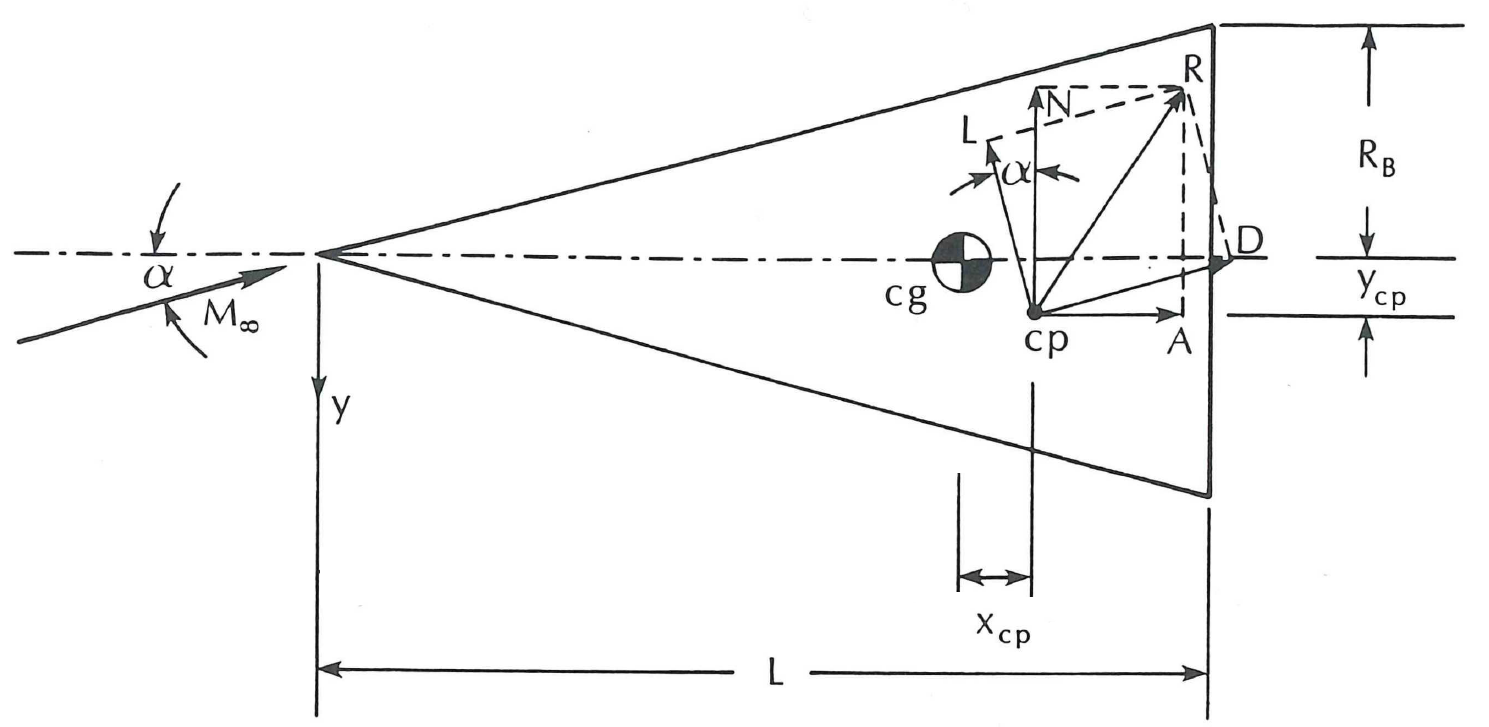
\includegraphics[width=0.7\textwidth]{./Figure/def_flap_distances}
%	\caption{Definition of flap moment arms}
%	\label{fig:flapstuff}
%\end{figure}
%By noting that both of these forces cause a moment
%\subsubsection{Control system design conclusions}
%From the previous sections one can conclude that all proposed concepts have their own strengths and weaknesses. In order to combine these it has been decided to combine \gls{cg}-shifting with
%
%
%***Moment or dalpha/dt that control systems (cg offset, thrusters, control surfaces) can create***\\
%***Weight estimate of each control system (per concept if needed)***\\

\subsection{Results \& conclusions}
\label{sec:astrores}
***intro***\\

\subsubsection{Atmospheric model}
\label{sec:astroatmos}
\begin{figure}[h]
	\centering
	\begin{subfigure}{0.45\textwidth}
	\centering
	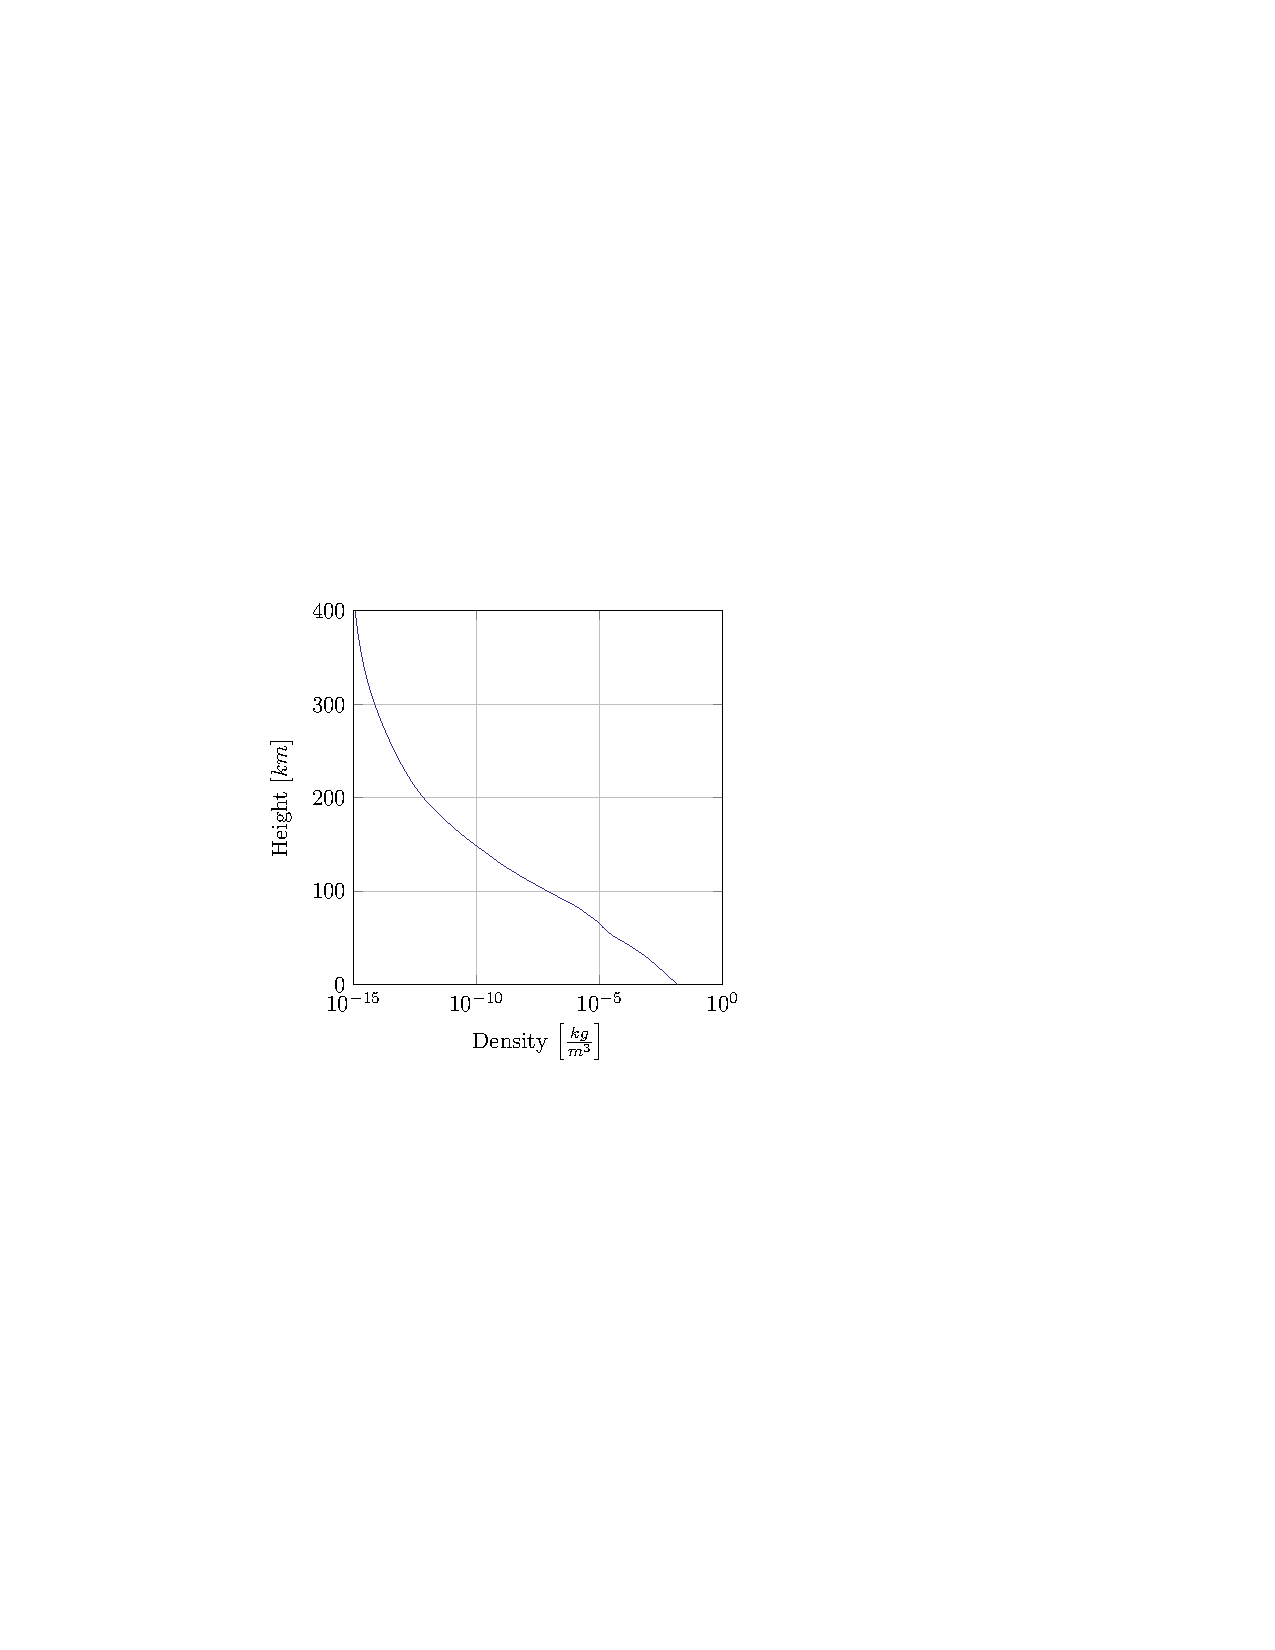
\includegraphics[trim={4cm 9.8cm 9cm 10cm},clip,width=0.9\textwidth]{Figure/atmos_model/density.pdf}
	\caption{The atmospheric density} 
	\label{fig:atmos_height_rho}
	\end{subfigure}
	\begin{subfigure}{0.45\textwidth}
	\centering
	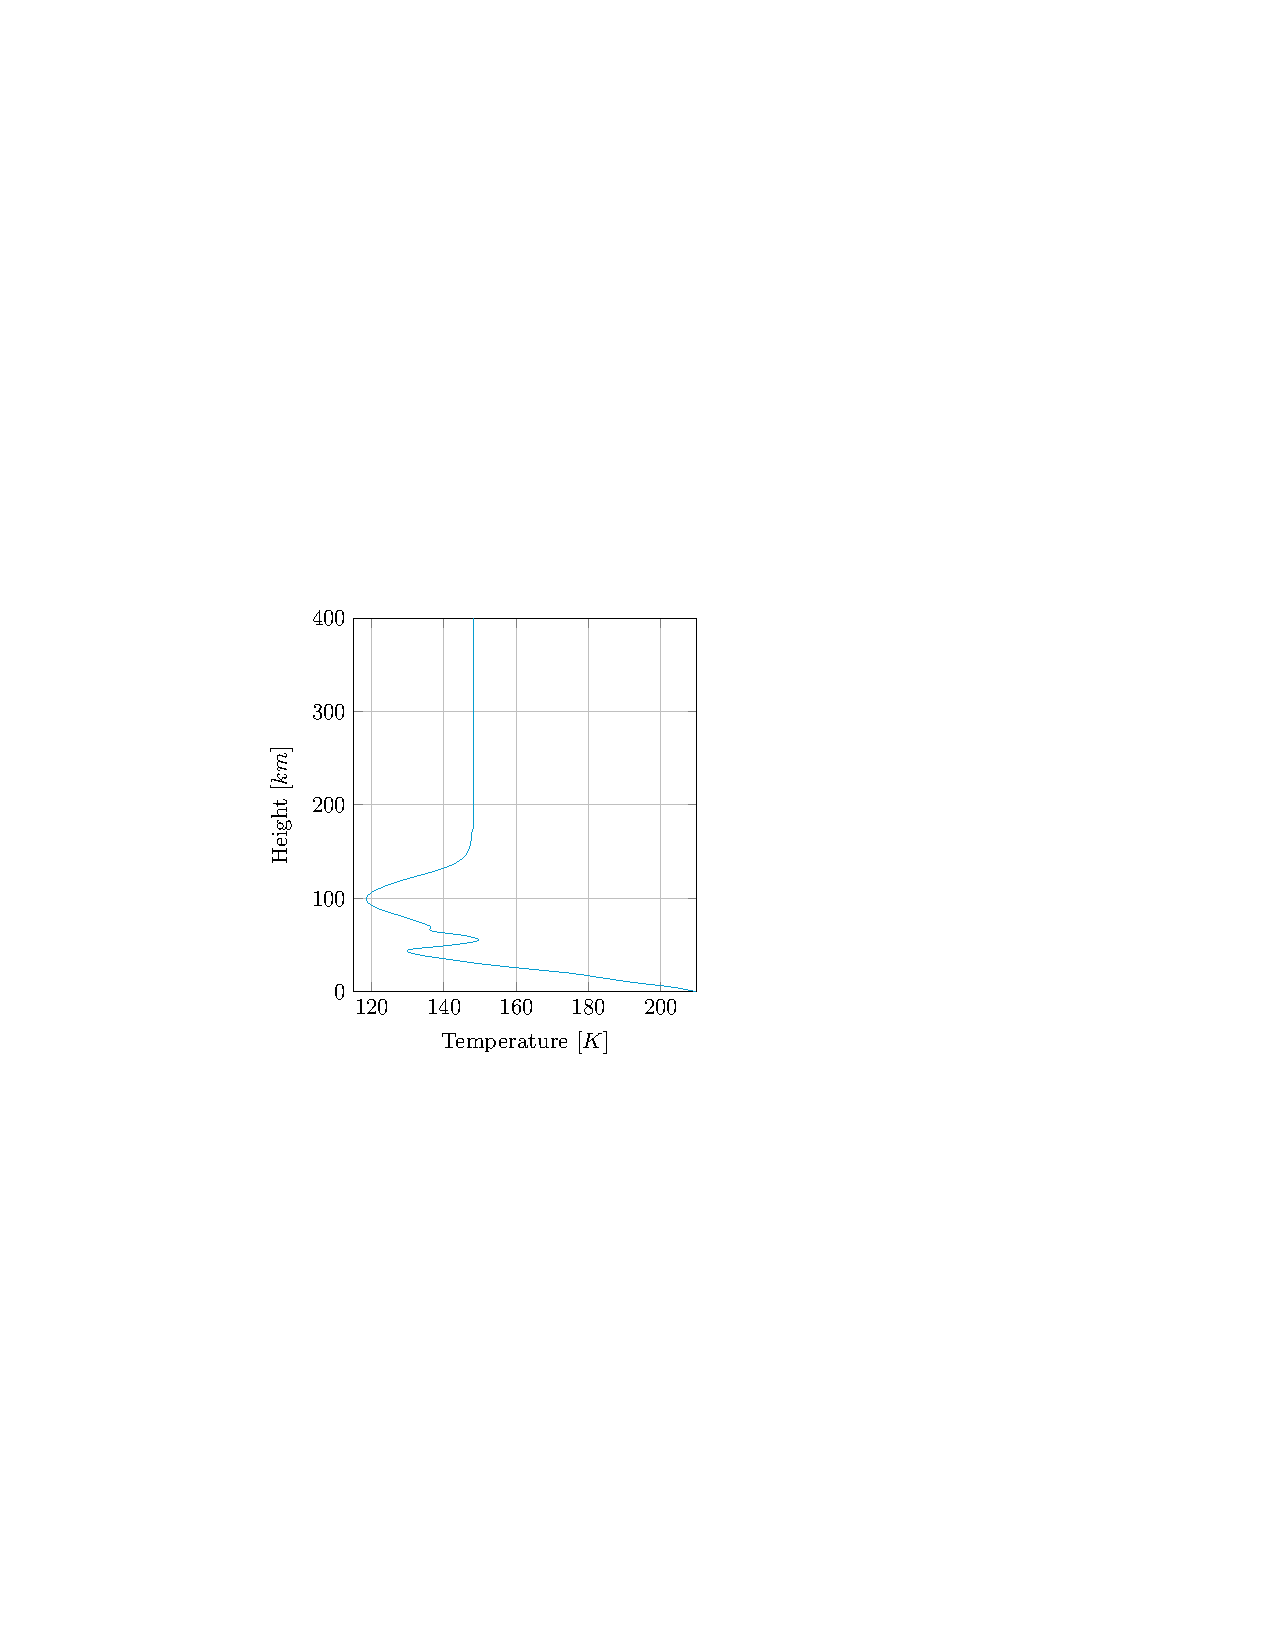
\includegraphics[trim={4cm 9.8cm 9cm 10cm},clip,width=0.9\textwidth]{Figure/atmos_model/temperature.pdf}
	\caption{The atmospheric temperature}
	\label{fig:atmos_height_T}
	\end{subfigure}
	\caption{The atmospheric properties for different heights}
	\label{fig:atmos_height}
\end{figure}

\begin{figure}[h]
	\centering
	\begin{subfigure}{0.9\textwidth}
	\centering
	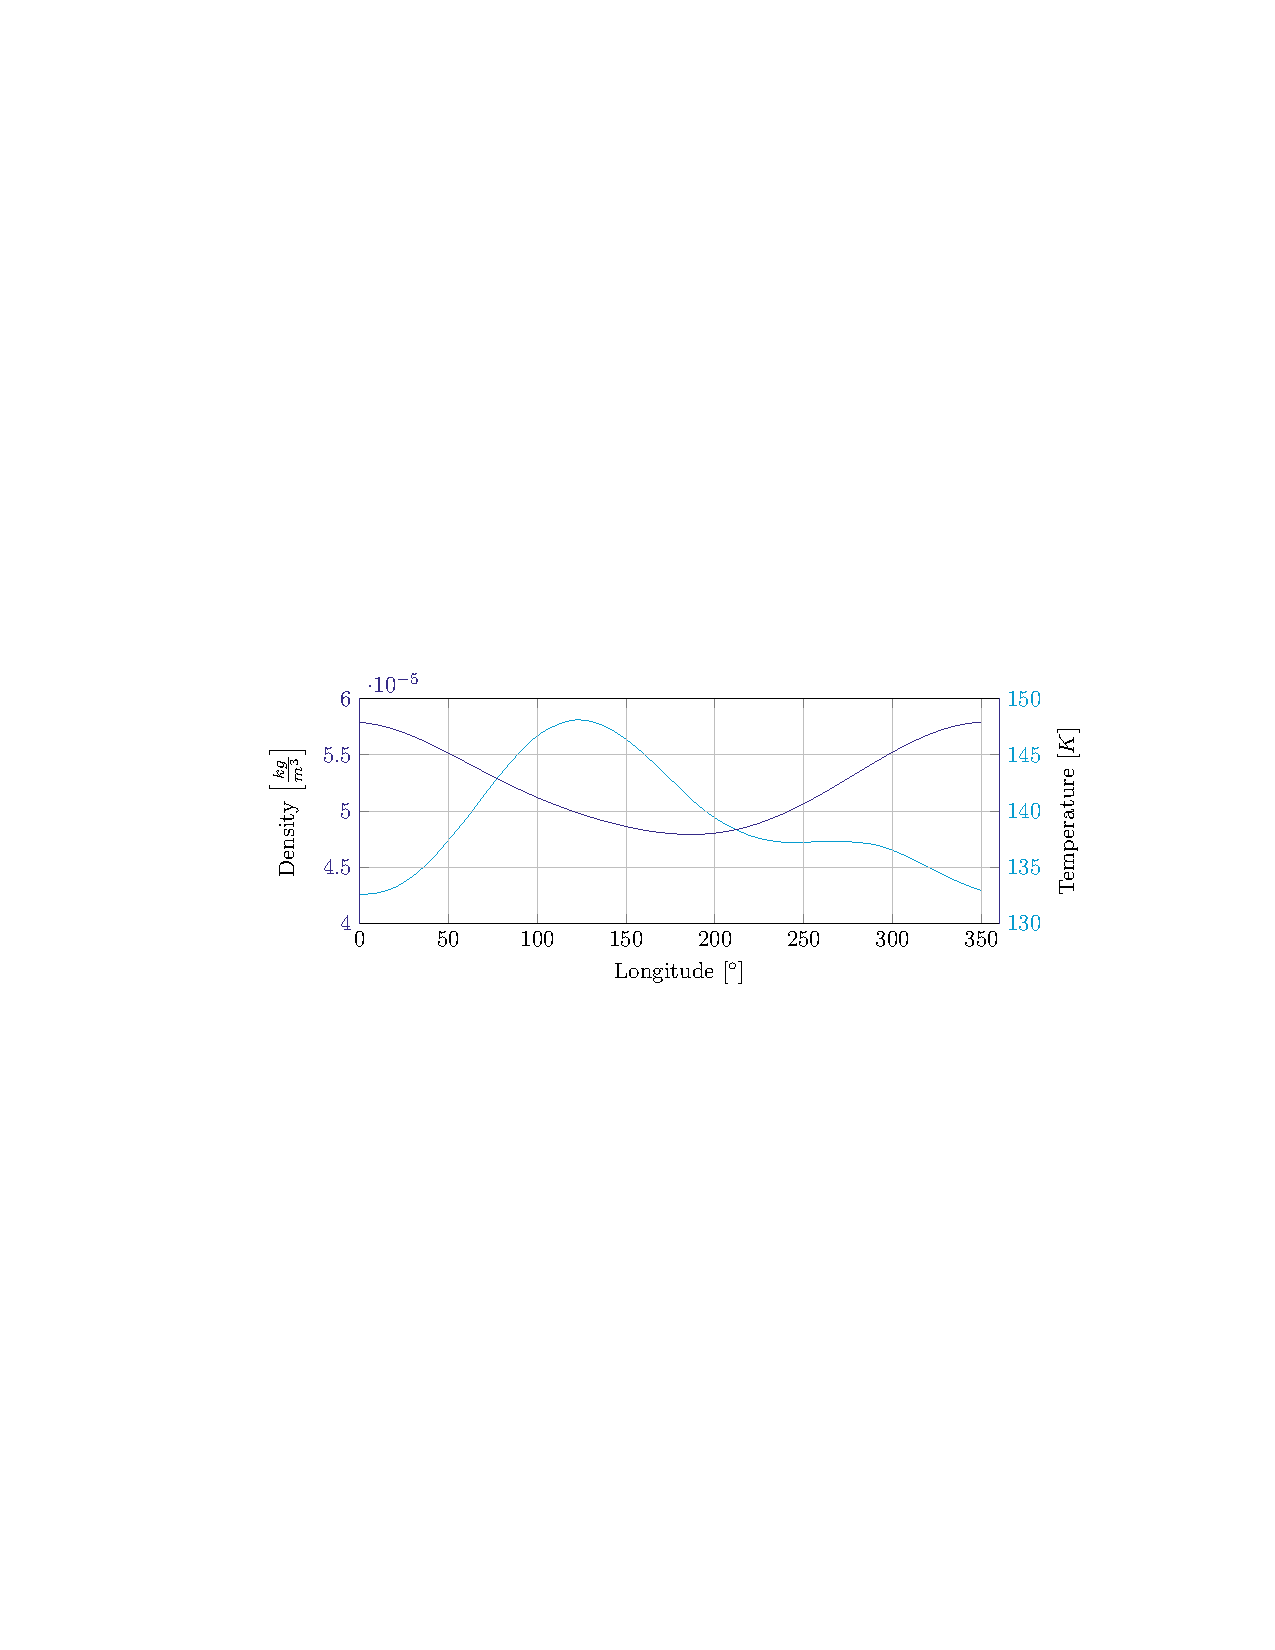
\includegraphics[trim={4.25cm 11cm 3.2cm 11cm},clip,width=0.9\textwidth]{Figure/atmos_model/lon_50.pdf}
	\caption{The atmospheric properties at $50$ $\left[km\right]$} 
	\label{fig:atmos_lon_50}
	\end{subfigure}
	\begin{subfigure}{0.9\textwidth}
	\centering
	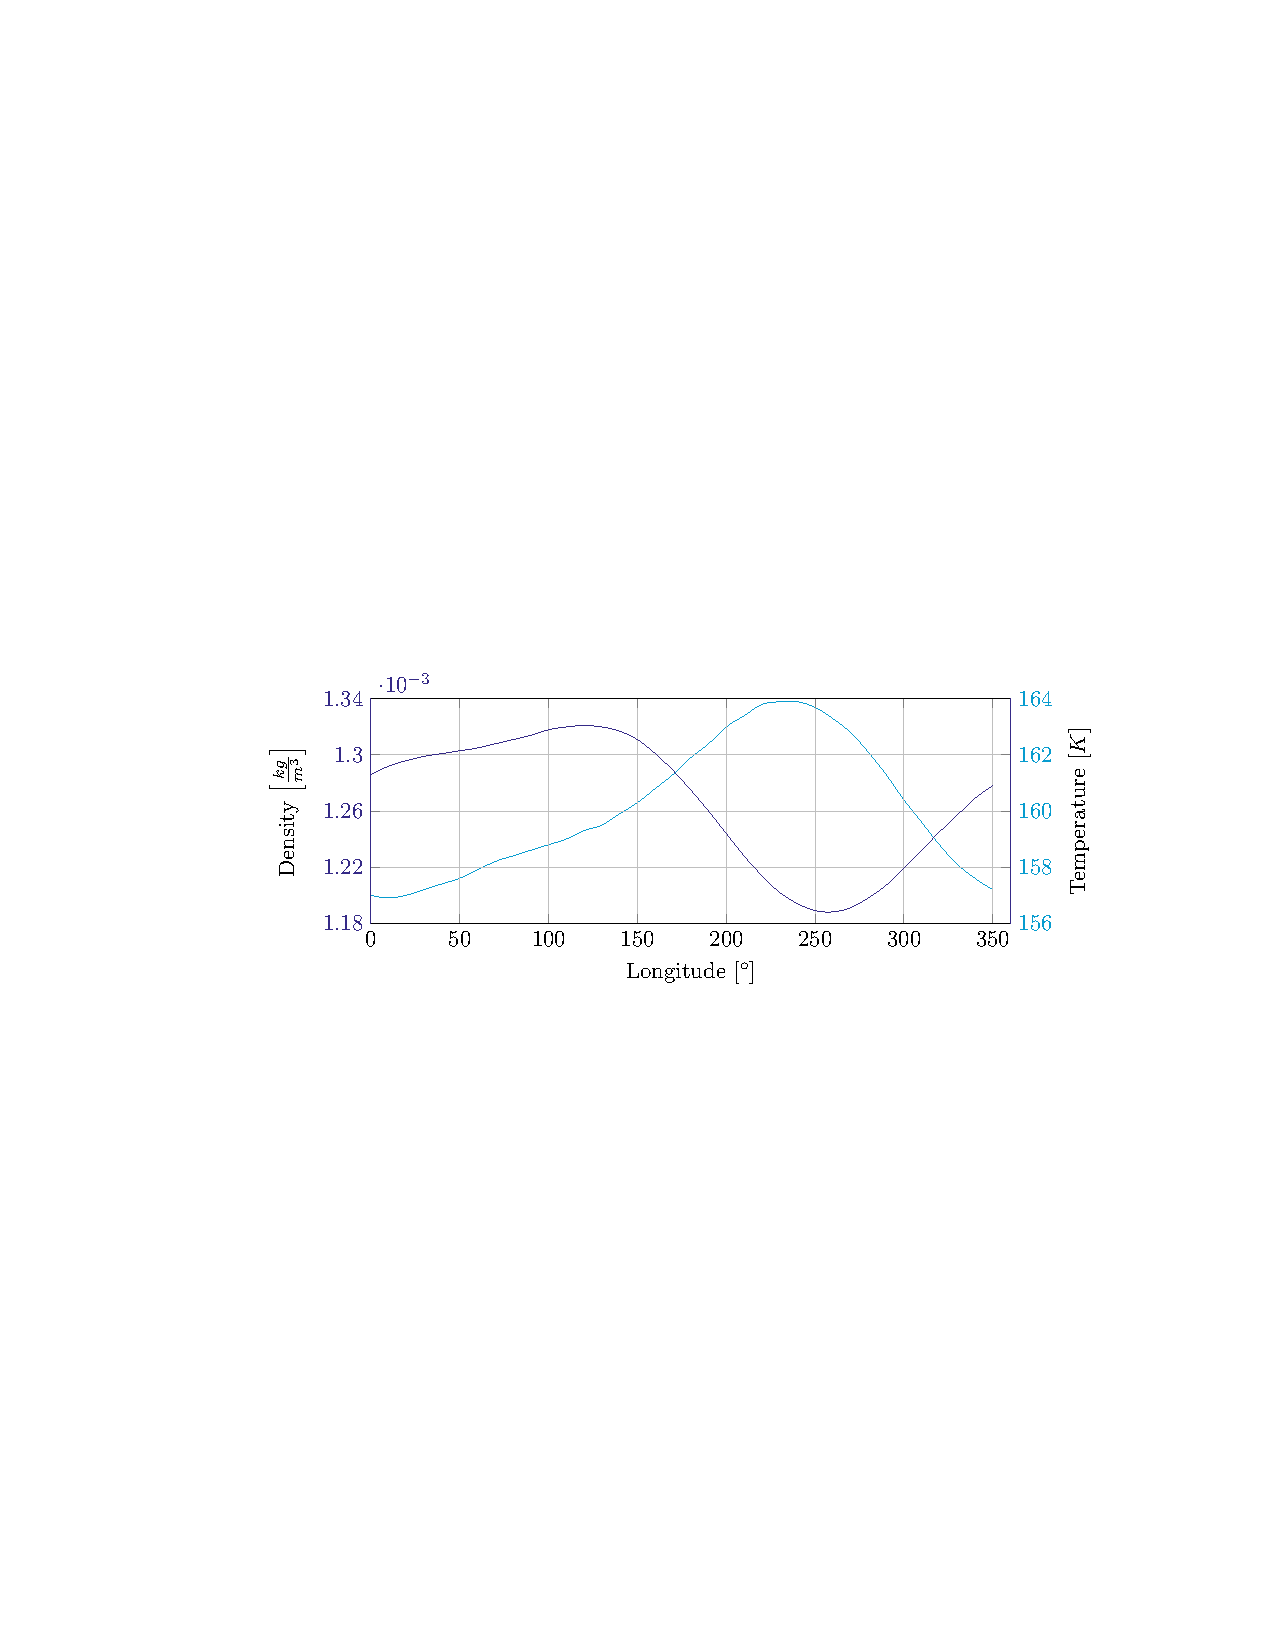
\includegraphics[trim={4.5cm 11cm 3.1cm 11cm},clip,width=0.9\textwidth]{Figure/atmos_model/lon_25.pdf}
	\caption{The atmospheric properties at $25$ $\left[km\right]$} 
	\label{fig:atmos_lon_25}
	\end{subfigure}
	\caption{The atmospheric properties for different heights at a latitude of 0 $\left[^\circ\right]$}
	\label{fig:atmos_lon}
\end{figure}

\subsubsection{Effect of \gls{sym:CL} and \gls{sym:CD} on deceleration}
\label{sec:astrodec}
***Two plots for CL and CD***\\

\subsubsection{A feasible trajectory and important output parameters over time}
\label{sec:astrorestraj}
***Plot of a trajectory***\\
***Plots of output variables for that particular trajectory***\\

\subsubsection{Required performance of the control system}
\label{sec:astroperfomance}
***Results of needed CLmax, dalpha/dt, dCL/dalpha***\\

\subsubsection{Conclusion on control system performance}
\label{sec:conclusion}
***Conclusion on which control system (implemented in which concept) can perform as such***\\
***Conclusion on weight the control systems will bring along***\\
***State values for in trade-off matrix***\\
